\ylDisplay{Kuulikesed} % Ülesande nimi
{Tundmatu autor} % Autor
{lahtine} % Voor
{2005} % Aasta
{G 4} % Ülesande nr.
{4} % Raskustase
{
% Teema: Elektrostaatika
\ifStatement
Seitse ühesugust laetud kuulikest laenguga $q$ on seotud omavahel samast materjalist võrdse algpikkusega elastsete niitidega ja saavad liikuda vaid ühes fikseeritud tasapinnas (vt joonist). Vahemaa kahe suvalise naaberkuulikese vahel tasakaalu olekus on $l$. Leidke tõmbepinged niitides.

\begin{center}
	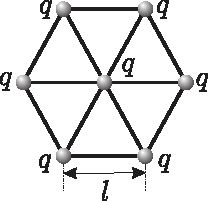
\includegraphics[width=0.35\linewidth]{2005-lahg-04-yl}
\end{center}
\fi


\ifHint
Sümmeetria tõttu mõjuvad kõikidele kuulidele radiaalsed sama väärtusega elektrostaatilised jõud, mis on niitide pingete poolt tasakaalustatud. Lisaks paneme tähele, et kuna niidid on identsed ning sama palju veninud, peavad kõikide niitide pinged võrdsed olema.
\fi


\ifSolution
\begin{center}
	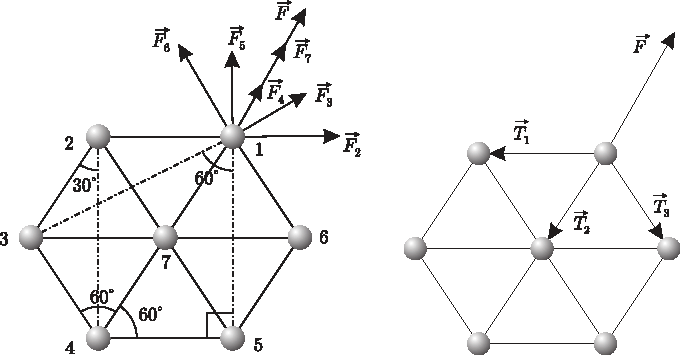
\includegraphics[width=\linewidth]{2005-lahg-04-lah}
\end{center}

Kõigepealt teeme kaks olulist tähelepanekut, lähtudes sümmeetria kaalutlustest:
\begin{enumerate}[wide=0pt, label={\arabic*)}]
	\item Keskmine kuul jääb paigale.
	\item Kõik 6 kuuli servades on samaväärsed, neile mõjuvate jõudude suurused on samad, kuid jõudude suunad on erinevad –--- nad langevad kokku sirgetega, mis ühendavad vastava kuulikese keskmise kuulikesega, ning, kuna laengud on samamärgilised, on suunatud keskmisest kuulikesest eemale.
\end{enumerate}

Märgime joonisel ühele äärmisele kuulikesele mõjuvad jõud (vt joonist). Leimae jõudude väärtused. Jõud $F_2$, $F_6$ ja $F_7$ mõjuvad kuulikesele 1, vastavalt, kuulikeste 2, 6 ja 7 poolt:
\[
F_2 = F_6 = F_7 = \frac{kq^2}{l^2}.
\]
Jõud $F_4$ mõjub kuulikesele 1 kuulikese 4 poolt:
\[
F_{4}=\frac{k q^{2}}{(2 l)^{2}}=\frac{k q^{2}}{4 l^{2}}.
\]
Jõud $F_3$ ja $F_5$ mõjuvad kuulikesele 1, vastavalt, kuulikeste 3 ja 5 poolt:
\[
F_{3}=F_{5}=\frac{k q^{2}}{\left(2 l \sin 30^{\circ}\right)^{2}}=\frac{k q^{2}}{(2 l \cdot \sqrt{3} / 2)^{2}}=\frac{k q^{2}}{3 l^{2}}.
\]
Summaarne jõu leiame projitseerides jõud radiaalsele teljele:
\[
\begin{aligned}
F&=F_{7}+F_{4}+2 F_{2} \cos 60^{\circ}+2 F_{3} \cos 30^{\circ}\\
&=\frac{k q^{2}}{l^{2}}+\frac{k q^{2}}{4 l^{2}}+2 \cdot 0,5 \cdot \frac{k q^{2}}{l^{2}}+2 \cdot \frac{\sqrt{3}}{2} \cdot \frac{k q^{2}}{3 l^{2}}=\frac{k q^{2}}{l^{2}}\left(1+\frac{1}{4}+1+\frac{\sqrt{3}}{3}\right)\\
&=\frac{k q^{2}}{l^{2}}\left(\frac{27+4 \sqrt{3}}{12}\right).
\end{aligned}
\]
Kuna tegu on ühesuguste niitidega, mis venisid sama palju (niitide alg- ja lõpppikkused on ühesugused), siis pinged kõigis niitides on võrdsed: 
\[
\vec{F}=\vec{T}_{1}+\vec{T}_{2}+\vec{T}_{3}, \quad\left|\vec{T}_{1}\right|=\left|\vec{T}_{2}\right|=\left|\vec{T}_{3}\right|.
\]
Siit:
\[
F = T + 2T \cos \SI{60}{\degree} = T (\num{1} + \num{2} \cdot \num{0,5}) = 2T.
\]
Seega niitides on pinge
\[
T=\frac{F}{2}=\frac{k q^{2}}{l^{2}}\left(\frac{27+4 \sqrt{3}}{24}\right).
\]
\fi
}